\subsection{Alloy to Java}
\subsubsection{Generating Java unit tests}
\paragraph{Translate Alloy signatures to Java classes}
To make Alloy solutions browsing easier, we translated every signature in the Alloy model into Java classes. For example, for the signatures $Method$ and $MethodCall$, we have the following classes:



\newsavebox{\firstlisting}
\begin{lrbox}{\firstlisting}% Store first listing
\begin{lstlisting}
abstract sig Method {
    paramTypes : seq Type,
    receiverType : Type
}

\end{lstlisting}
\end{lrbox}
\newsavebox{\secondlisting}
\begin{lrbox}{\secondlisting}% Store second listing
\begin{lstlisting}
sig MethodCall extends CallWithNext{
    receiver : Object,
    method : Method,
    params : seq Object
}
\end{lstlisting}
\end{lrbox}

\begin{figure}[h]
{\usebox{\firstlisting}} \hfill%
{\usebox{\secondlisting}}
\end{figure}

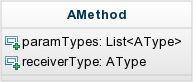
\includegraphics{method.png}
\hfill
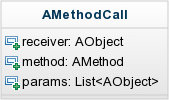
\includegraphics{methodcall.png}



\paragraph{Modelizing Alloy instances in Java}
Using Alloy Analyzer we execute the generated Alloy source code. Alloy Analyzer generates all possible instances.
Each instance is a solution, we can obtain a solution using A4Solution object. A4Solution object has a method \textit{satisfiable} to check if the solution is valid and a method \textit{next} to go the next possible solution.

\paragraph{Generating tests}
In order to generate the code of Java unit tests, we used CodeModel, which allows us to generate Java classes in a simple way.\\
We browse Java modelized solution and generate the variables used to call methods and the variables passed as methods parameters.\\
For each solution we use the execution trace.
Firstly, we initalize all the necessary types for the receiver method, then all the veriables that will be used in parameters. \\
If an exception occurs during the execution of the tests, its stack trace is logged in a file, and the number of different exceptions thrown is written in the file.\\

\begin{algorithm}[H]
\SetAlgoLined
\KwData{Alloy instance modelized in Java}
\KwResult{Java unit test}
 \ForEach{Alloy Instance modelized in Java}{
		Get the head of method calls list\;
		\While{ methods calls are not finished}{
 		 Create method signature\;
 		 Add $org.Junit.Test$ annotation \;
		 Add $Throw Exception$ to method signature\;
		 Create a $try catch$ block\;
		 Inside the $try$ block:\{\\
	     - Declare all variables\\
	     - Call constructors\\
	     - Add method calls with the necessary parameters\\
		 \}\;
		 Inside the $catch$ block:\{\\
	     - Log the exception in a file\\
	     - Rethrow it\\
		 \}\;
 	}}
~\\
\caption{How to translate an Alloy instance modelized in Java into Java unit tests}
\end{algorithm}
\bigskip
\bigskip
An example of the results output:

\lstset{ %
  backgroundcolor=\color{white},   % choose the background color
  basicstyle=\footnotesize,        % size of fonts used for the code
  breaklines=true,                 % automatic line breaking only at whitespace
  captionpos=b,                    % sets the caption-position to bottom
  commentstyle=\color{mygreen},    % comment style
  escapeinside={\%*}{*)},          % if you want to add LaTeX within your code
  keywordstyle=\color{red!40!black},    % keyword style
  stringstyle=\color{mymauve}, 
  upquote=true    % string literal style
}

\begin{lstlisting}[language=java]
@BeforeClass
public static void initExceptionBuilder() throws IOException {
    ExceptionLogger.initLogFile();
}
\end{lstlisting}

\begin{lstlisting}[language=java]
@Test
public void test0() throws Exception {
  try {
  			
  }catch(java.lang.Exception x){
    ExceptionLogger.logException(x);
    throw(x);
  }
}
\end{lstlisting}

\begin{lstlisting}[language=java]
@AfterClass
public static void closeExceptionBuilder() throws IOException {
    ExceptionLogger.closeLogFile();
}
\end{lstlisting}

